\documentclass[a4paper,11pt]{article}
\usepackage{times}
\usepackage{ogonek} % Dąbkowski
\hyphenation{Acad-e-my}
\usepackage{pdfpages}
\pdfinclusioncopyfonts=1
\usepackage[utf8]{inputenc}
        \usepackage{hyperref}
        \hypersetup{colorlinks=false, pdfborder={0 0 0}}
        \setcounter{page}{280}
        \begin{document}

\newcommand\formatauthor[2]{\begin{tabular}[t]{@{}c@{}}
  {\LARGE#1\strut}\\
  {\small#2\strut}\\
  \rule{\dimexpr0.5\linewidth-1em}{0pt}
  \end{tabular}\xhfill\ignorespaces}
\newcommand\xhfill{\hspace{1em plus 1fill}}
\thispagestyle{empty}

\begin{center}
  {\huge\bfseries Obligatory Control and Event Structure in Kavalan\par}

  \bigskip

~\\
\begingroup
\setlength{\leftskip}{0pt plus 1fill}
\setlength{\rightskip}{0pt plus 1fill}
\setlength{\parindent}{0pt}
\setlength{\parfillskip}{0pt}
  \formatauthor{Dong-yi Lin}{\begin{tabular}{@{}c@{}}Ghent University\end{tabular}}

\par\endgroup

  \vspace*{8ex}

  Proceedings of the 21st International Conference on\par Head-Driven Phrase Structure Grammar

  \bigskip

  University at Buffalo

  \medskip

  Stefan Müller (Editor)

  \medskip

  2014

  \medskip

  CSLI Publications

  \medskip

  pages 280--298

  \medskip

  \url{http://csli-publications.stanford.edu/HPSG/2014}
\end{center}
\vfill

\noindent



\vfill
\noindent
% APA Style
Lin, Dong-yi. 2014. Obligatory Control and Event Structure in Kavalan. In Müller, Stefan (Ed.), \emph{{Proceedings of the 21st International Conference on Head-Driven Phrase Structure Grammar, University at Buffalo}}, 280--298. Stanford,
CA: CSLI Publications. \hfill\href{http://creativecommons.org/licenses/by/4.0/}{\includegraphics[height=.75em]{Includes/ccby.eps}}

\newpage
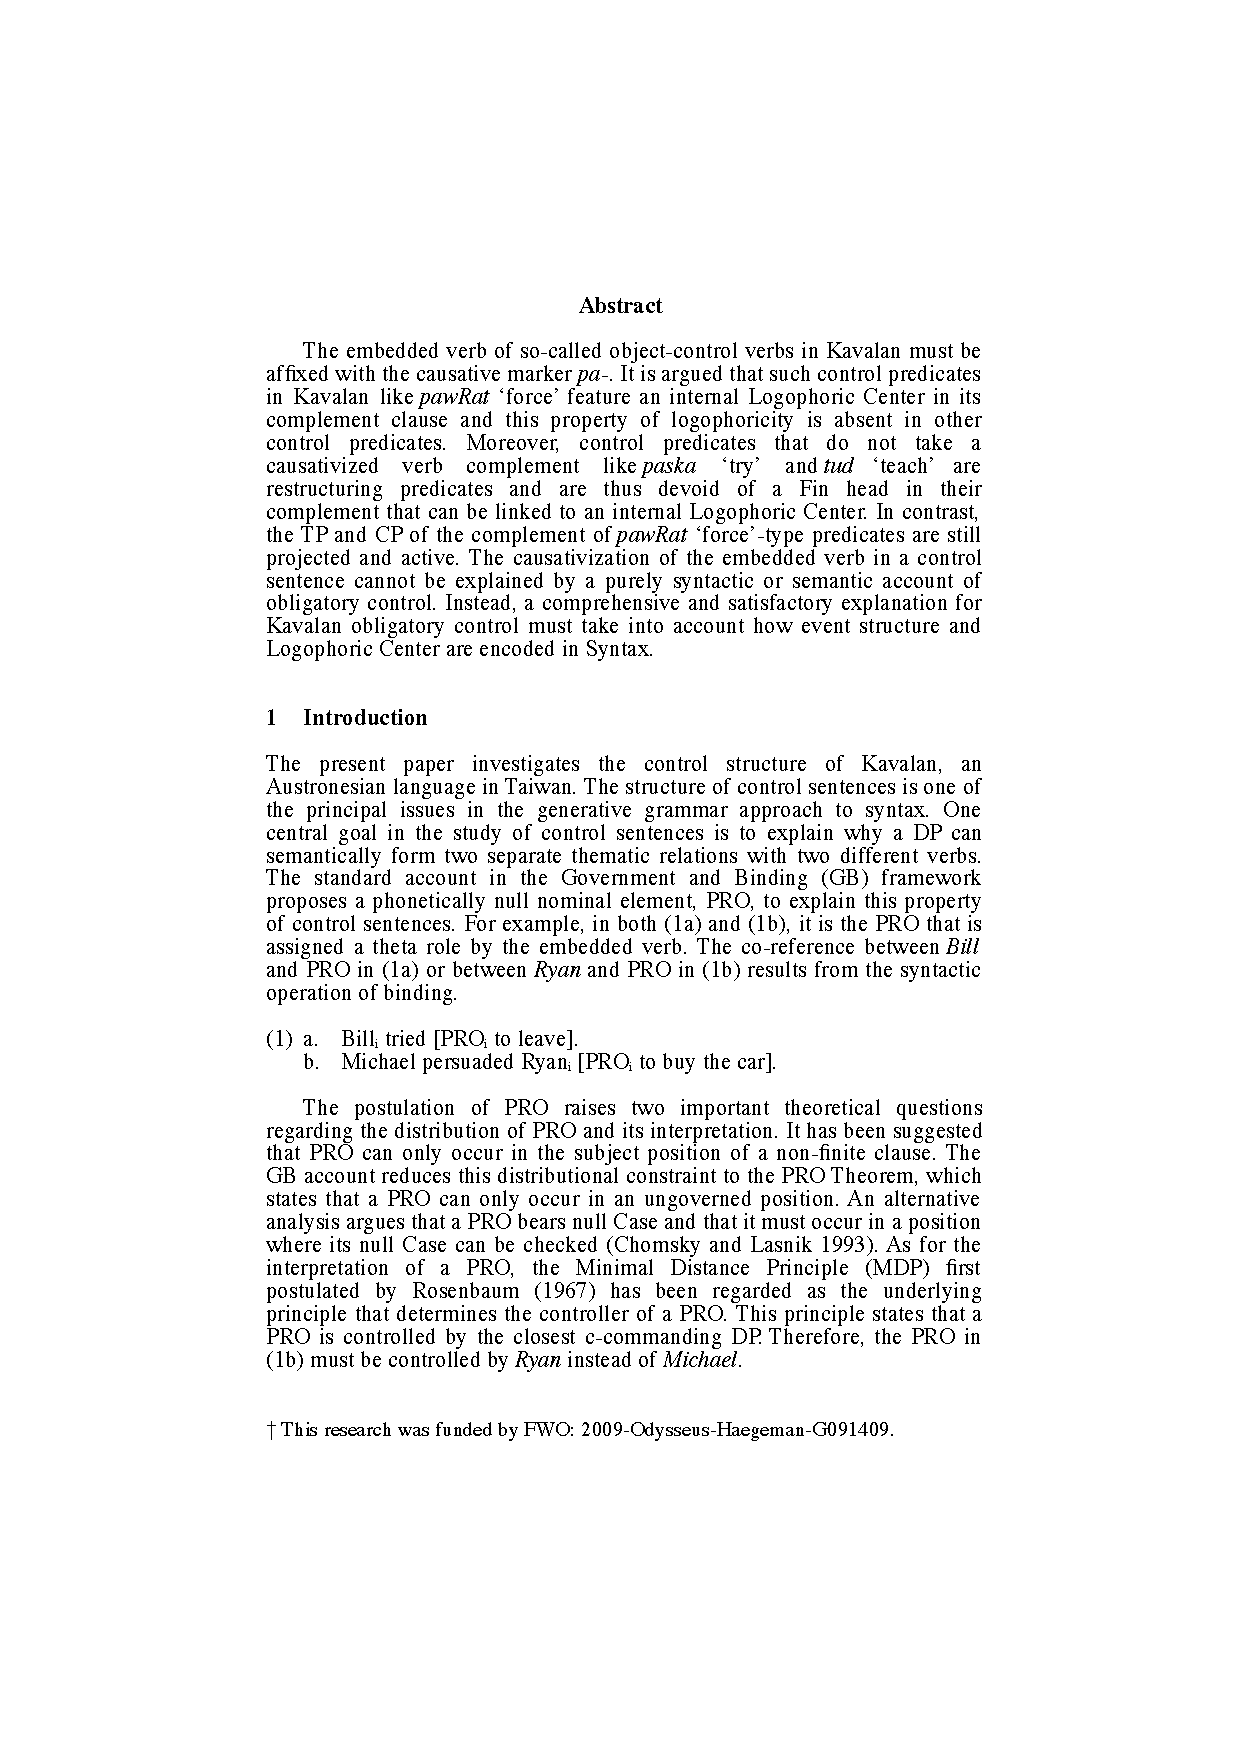
\includepdf[pages=-,pagecommand=\thispagestyle{plain}]{Includes/lin.pdf}
        \end{document}
